\documentclass{beamer}
\usepackage[latin1]{inputenc}
\usepackage{amsfonts}
\usepackage{epsfig}
\usepackage{hyperref}
\usepackage{multicol}
\usepackage{graphicx}
\usepackage{color}
\usetheme{Warsaw}
\title[The Tempest \hspace{15em} \insertframenumber / \inserttotalframenumber]{Colonization in The Tempest and its Afterlives}

\author {Ravi Bhoraskar}
\begin{document}
\begin{frame}[plain]
\titlepage
\begin{center}
\begin{figure}[htp]
  \begin{center}
    \centering
    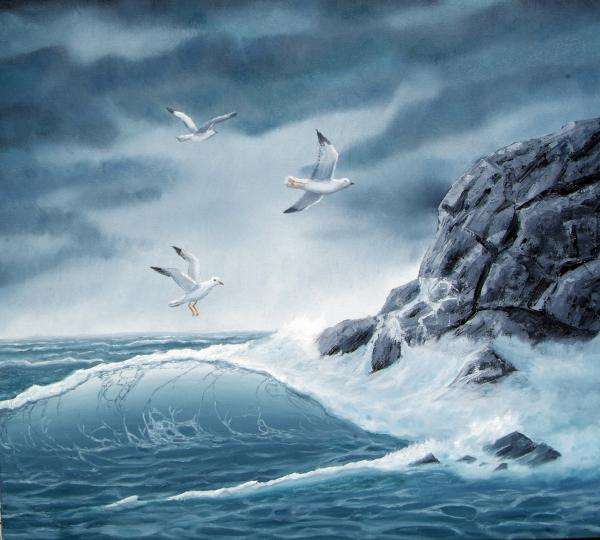
\includegraphics[scale=0.17]{title.jpg}
  \end{center}
\end{figure}
under guidance of\\
Prof. Sudha Shastri\\
IIT Bombay
\end{center}
\end{frame}
\begin{frame}{Outline}
  \begin{multicols}{2}
  \tableofcontents  
  \end{multicols}
\end{frame}
\section{Introduction}
\subsection{A brief history of Colonization}
\begin{frame}{A brief history of British Colonization}
  \begin{columns}[c]
    \column{.6\textwidth}
  \begin{itemize}
  \item \textbf{1492} Columbus discovered America (mistook it for India)
  \item \textbf{1497} Henry VII commissions John Cabot; First Englishman in America
   %No colonization so far, just trade. John Cabot's ship disappeared in his second voyage.
  \item \textbf{1576 onwards} Early claims of land in the name of queen
  \item \textbf{1607} Colonization of America started, with \emph{Virginia Company} creating colony at Jamestown, Virginia
    %Parallels with the colonial discourse prophetic, rather than descriptive
  \end{itemize}
  \column{.4\textwidth}
    \begin{figure}[htp]
      \begin{center}
        \centering
        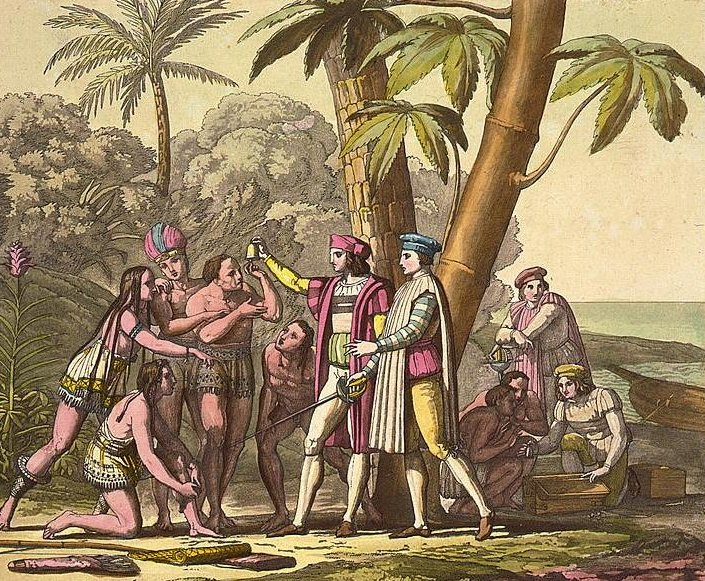
\includegraphics[scale=0.29]{columbus.jpg}
      \end{center}
    \end{figure}
    \end{columns}
\end{frame}

\begin{frame}{The Sea Venture incident}
  \begin{columns}[c]
    \column{.4\textwidth}
    \begin{figure}[htp]
      \begin{center}
        \centering
        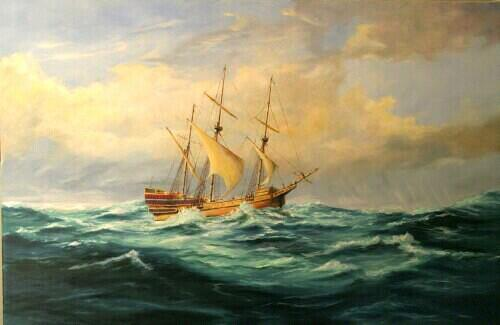
\includegraphics[scale=0.29]{seaventure.jpg}
      \end{center}
    \end{figure}
    \footnotesize{\emph{The Sea Venture in a heavy Sea in 1609,} painting by Christopher Grimes}
    \column{.6\textwidth}

  \begin{itemize}
  \item \emph{Sea Venture} commissioned in 1609 to deliver supplies to the Jamestown colony
  \item Set sail on June 20; Ran into storm and sank on July 24
  \item All 150 passengers land safely ashore, onto a reef in Bermuda
  \item Stranded for 9 months; built 2 new boats; sailed to Virginia; most saved
  \item William Strachey wrote accounts, which supposedly inspired The Tempest
  \end{itemize}
  \end{columns}
\end{frame}


\begin{frame}{The Tempest}
  See video 'The Tempest in a minute'
\end{frame}

\subsection{The Tempest}
\begin{frame}{The Tempest}
  \begin{itemize}
    \item Shakespeare's last play; written in 1610-11
    \item Based in the Mediterranean, but the island seems more like the \emph{New World}
    \item Strict observation of the three unities, in contrast to other Shakespeare's plays 
    \item Prospero an image of Shakespeare, with his renunciation of magic depicting Shakespeare's farewell to the stage
    \item Colonization had just started, hence parallels with the colonial discourse prophetic, rather than descriptive
  \end{itemize}
\end{frame}

\subsection{The Afterlives}
\begin{frame}{The Afterlives}
  \begin{enumerate}
  \item \textbf{Neil Gaiman's \emph{The Tempest}}
    \begin{itemize}
    \item \textbf{1997} Last book of \emph{The Sandman} series, part of \emph{The Wake}
    \end{itemize}
  \item \textbf{Charles and Mary Lamb's \emph{Tales from Shakespeare}}
    \begin{itemize}
    \item \textbf{1807} Written as an abridged version of Shakespeare for children
    \item Attempts to be a reproduction, but is an afterlife, due to cultural sensibilities of its times
    \end{itemize}
  \item \textbf{The Tempest: Graphic Novel}
    \begin{itemize}
    \item \textbf{2009} Retains the original text, but adds pictures
    \end{itemize}
  \end{enumerate}
\end{frame}

\section{Postcolonial Theory and The Tempest}
\subsection{Prospero and Postcolonialism}
\begin{frame}{Postcolonial Theory and The Tempest}
  \emph{``Postcolonialism is intellectual discourse that consists of reactions to, and analysis of, the cultural legacy of colonialism and imperialism.''}
  \begin{itemize}
    \item The tempest has been viewed through a lens of postcolonial theory
    \item Prospero, earlier seen as a \emph{benevolent God}, has flaws
      \begin{itemize}
      \item Seen as patriarchal, colonialist, sexist and racist
      \item \textbf{Ariel} A companion or familiar. Desires freedom
      \item \textbf{Caliban} A slave. Often mistreated, and used for menial tasks. Justified due to his attempted rape on Miranda
      \item \textbf{Miranda} Prospero's daughter. Prospero is protective, often domineering. Finds it hard to let her go
      \end{itemize}
  \end{itemize}
  \end{frame}
\subsection{Caliban}
  \begin{frame}{Caliban and the Colonial Discourse 1/2}
    \begin{itemize}
    \item Sycorax's son, original inhabitant of the island, at peace with nature; Parallels with Indians
    \item \textcolor{red}{\emph{``And then I lov'd thee, and show'd thee all the qualities o' th' isle .....Cursed be I that did so!.....For I am all the subjects that you have, which first was mine own King''}}
    \item Seen as savage, uncivilized. Prospero sees the need to \emph{civilize} him; White man's burden
    \end{itemize}
  \end{frame}
  \begin{frame}{Caliban and the Colonial Discourse 2/2}
    \begin{itemize}
    \item Attempted rape of Miranda \textcolor{red}{\emph{``Would't had been done! Thou didst prevent me; I had peopled else this isle with Calibans''}} Wishes to dominate what he sees are rightfully his own island. Colonizer sees it as a threat to his own dominance, hence subjugates him
    \item \textcolor{red}{\emph{``You taught me language; And my profit on't is, I know how to curse''}}; Postcolonial literature often in the colonizer's language, though critical of colonization
    \item Stephano and Trinculo pour wine down his throat and reduce him to a boot-licking slave; Colonization of the worst kind
    \end{itemize}
  \end{frame}

  \begin{frame}{More Caliban}
      Charles Lamb says \textcolor{red}{\emph{...a strange misshapen thing, far less human in form than an ape.... would have been very kind to him, but the bad nature, which Caliban inherited from his mother Sycorax, would not let him learn anything good or useful: therefor he was employed like a slave, to fetch wood, and do the most laborious offices;}}

        The Tempest: Graphic Novel depicts caliban as a non-human, almost demon-like creature. <insert picture>

        Attempts to dehumanize him, so as to not elicit sympathy, and justify Prospero's conduct. Shakespeare is more neutral, and shows Caliban's POV too.
  \end{frame}

  \section{Neil Gaiman's The Tempest}
  \begin{frame}{Neil Gaiman's The Tempest}
    \begin{itemize}
      \item Neil Gaiman : Comic Books :: Shakespeare : Drama
      \item Last book of the Sandman series, last play by Shakespeare, Gaiman sees himself in Shakespeare, Shakespeare sees himself in Prospero
      \item Highlights the labours of writing; writing as a chore instead of it being a creative process
      \item Comments on universality and immortality of Shakespeare
    \end{itemize}
  \end{frame}
  
  \begin{frame}{Graphic Novel vs Play}
  \end{frame}
  
  \begin{frame}{The Afterlife}
    \begin{itemize}
  \item An afterlife may seek to fill in gaps in the original text
  \item Might attempt to explain or justify why certain things are the way they are in the original text
  \item Justification required when the cultural context changes -- e.g. in a postcolonial world
  \item Hob Gadling's (another Sandman character) remorse over slave trade is congruent to Afterlives justifying aspects of the original text
    \end{itemize}
  \end{frame}
  
  \begin{frame}{Labours of Writing}
    Some pictures from The Wake, with commentary
  \end{frame}

  \begin{frame}{Shakespeare and Prospero}
    Discuss parallels between Shakespeare and  Prospero, Judith and Miranda (with pictures)
  \end{frame}

  \begin{frame}{Ben Johnson, and reaction to Shakespeare}
    Discuss how Shakespeare was taken in his own time, with mention of Ben Johnson in the Graphic Novel. Discuss Shakespeare's immortality, and was it just a fluke?    
  \end{frame}
  
  \begin{frame}{Universality of Shakespeare}
    The conversation with Ben Johnson, in which Shakespeare says that all one needs to appeal to people, is to be a human being, and to understand human emotions.
    Here, also discuss the Meredith Anne Skura's paper, that says that the parallels to colonization in The Tempest are coincidental, and its all due to Shakespeare's acute understanding of human nature
  \end{frame}

  \section{Conclusion}
  \begin{frame}{Conclusions}
    \end{frame}
\end{document}
